\documentclass[aspectratio=169]{beamer}
\usetheme{Madrid}

\setbeamertemplate{navigation symbols}{}
\setbeamertemplate{headline}{}

\usepackage[T1]{fontenc}
\usepackage{graphicx}
\graphicspath{{figures/}{img/}}
\usepackage{tikz}
\usetikzlibrary{shapes,arrows,positioning,calc}
\usepackage{booktabs}

\title{Voice-LLM Workbench}
\subtitle{Part II Progress Presentation}
\author{Vedaangh Rungta}
\institute{University of Cambridge}
\date{February 2026}

\begin{document}

\begin{frame}[plain]
\titlepage
\end{frame}

\begin{frame}{Introduction}
\centering
\vspace{0.5em}
{\Large\textbf{Goal:} Build a platform to scalably train and deploy speech}\\[0.3em]
{\Large on top of existing open-source LLM backbones.}

\vspace{1em}
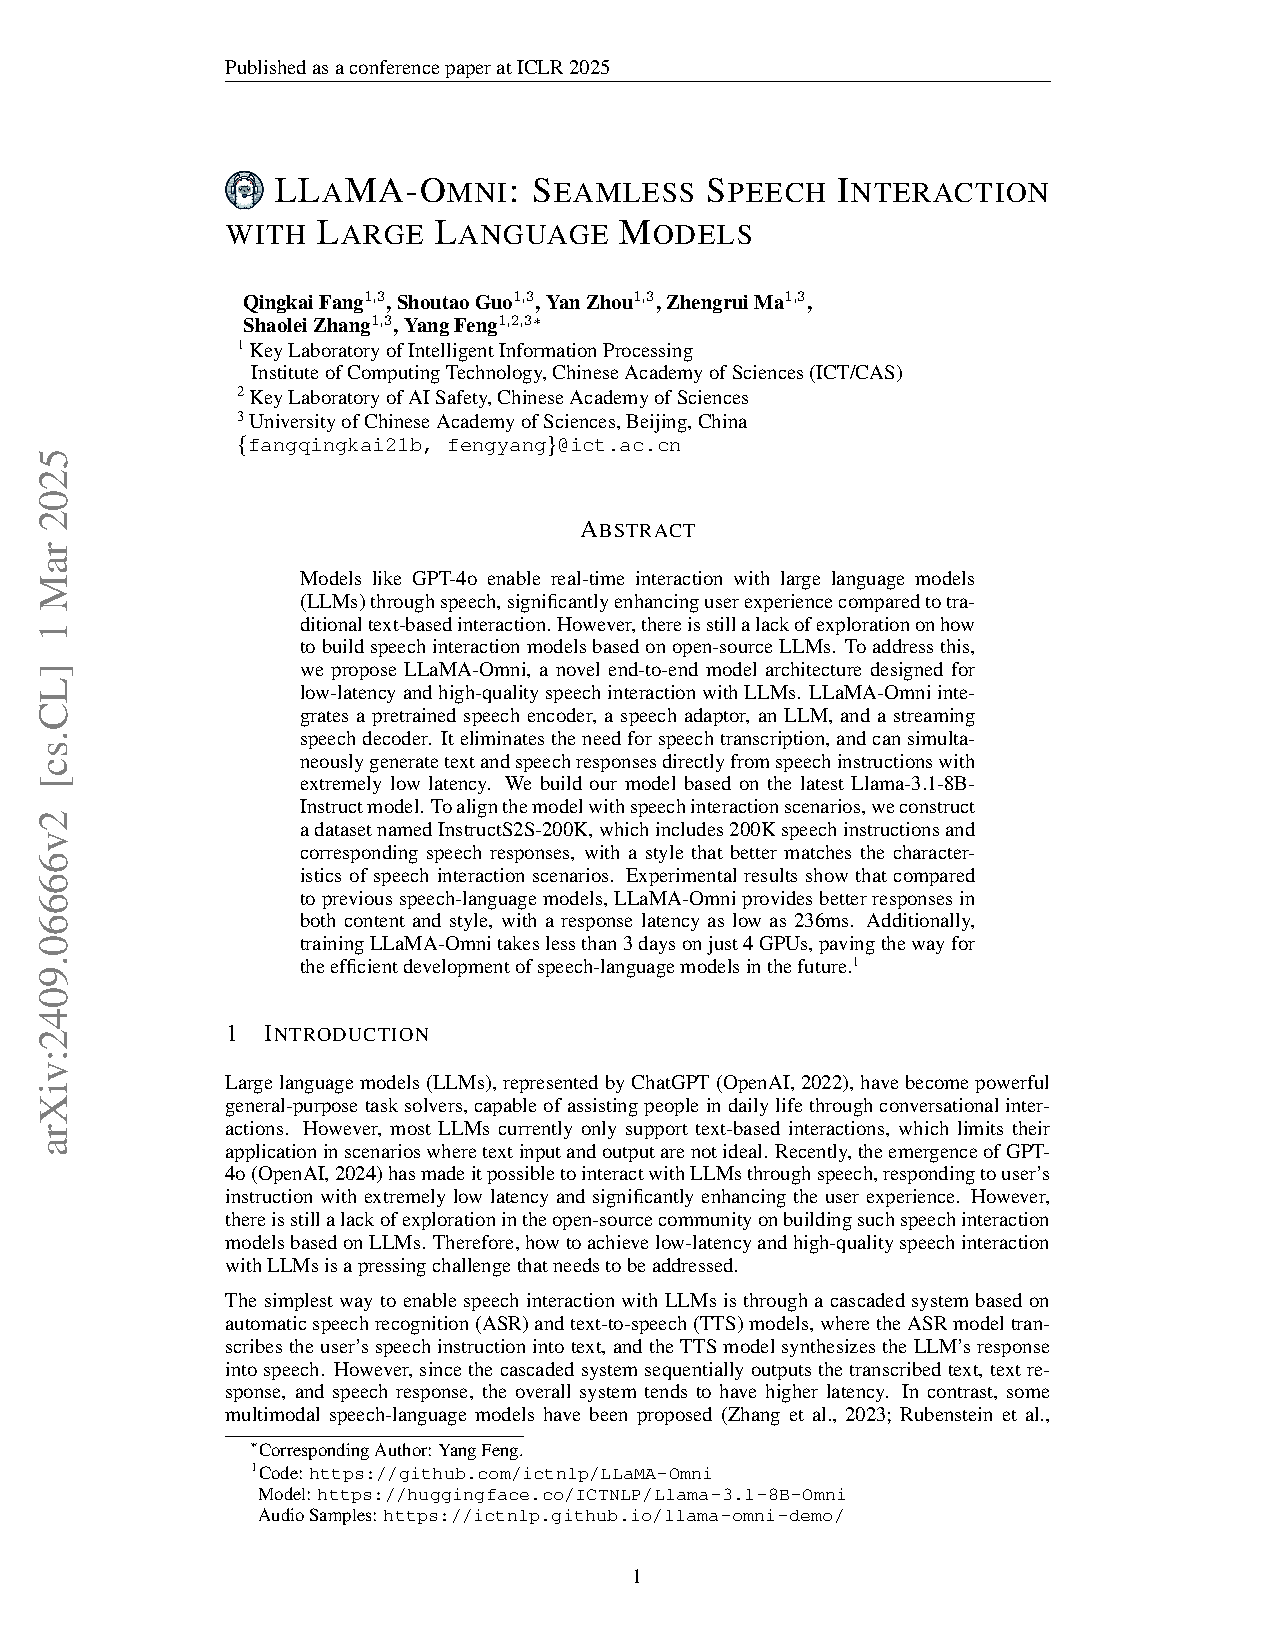
\includegraphics[height=4.8cm,page=1]{llama_omni_paper.pdf}
\hspace{1cm}
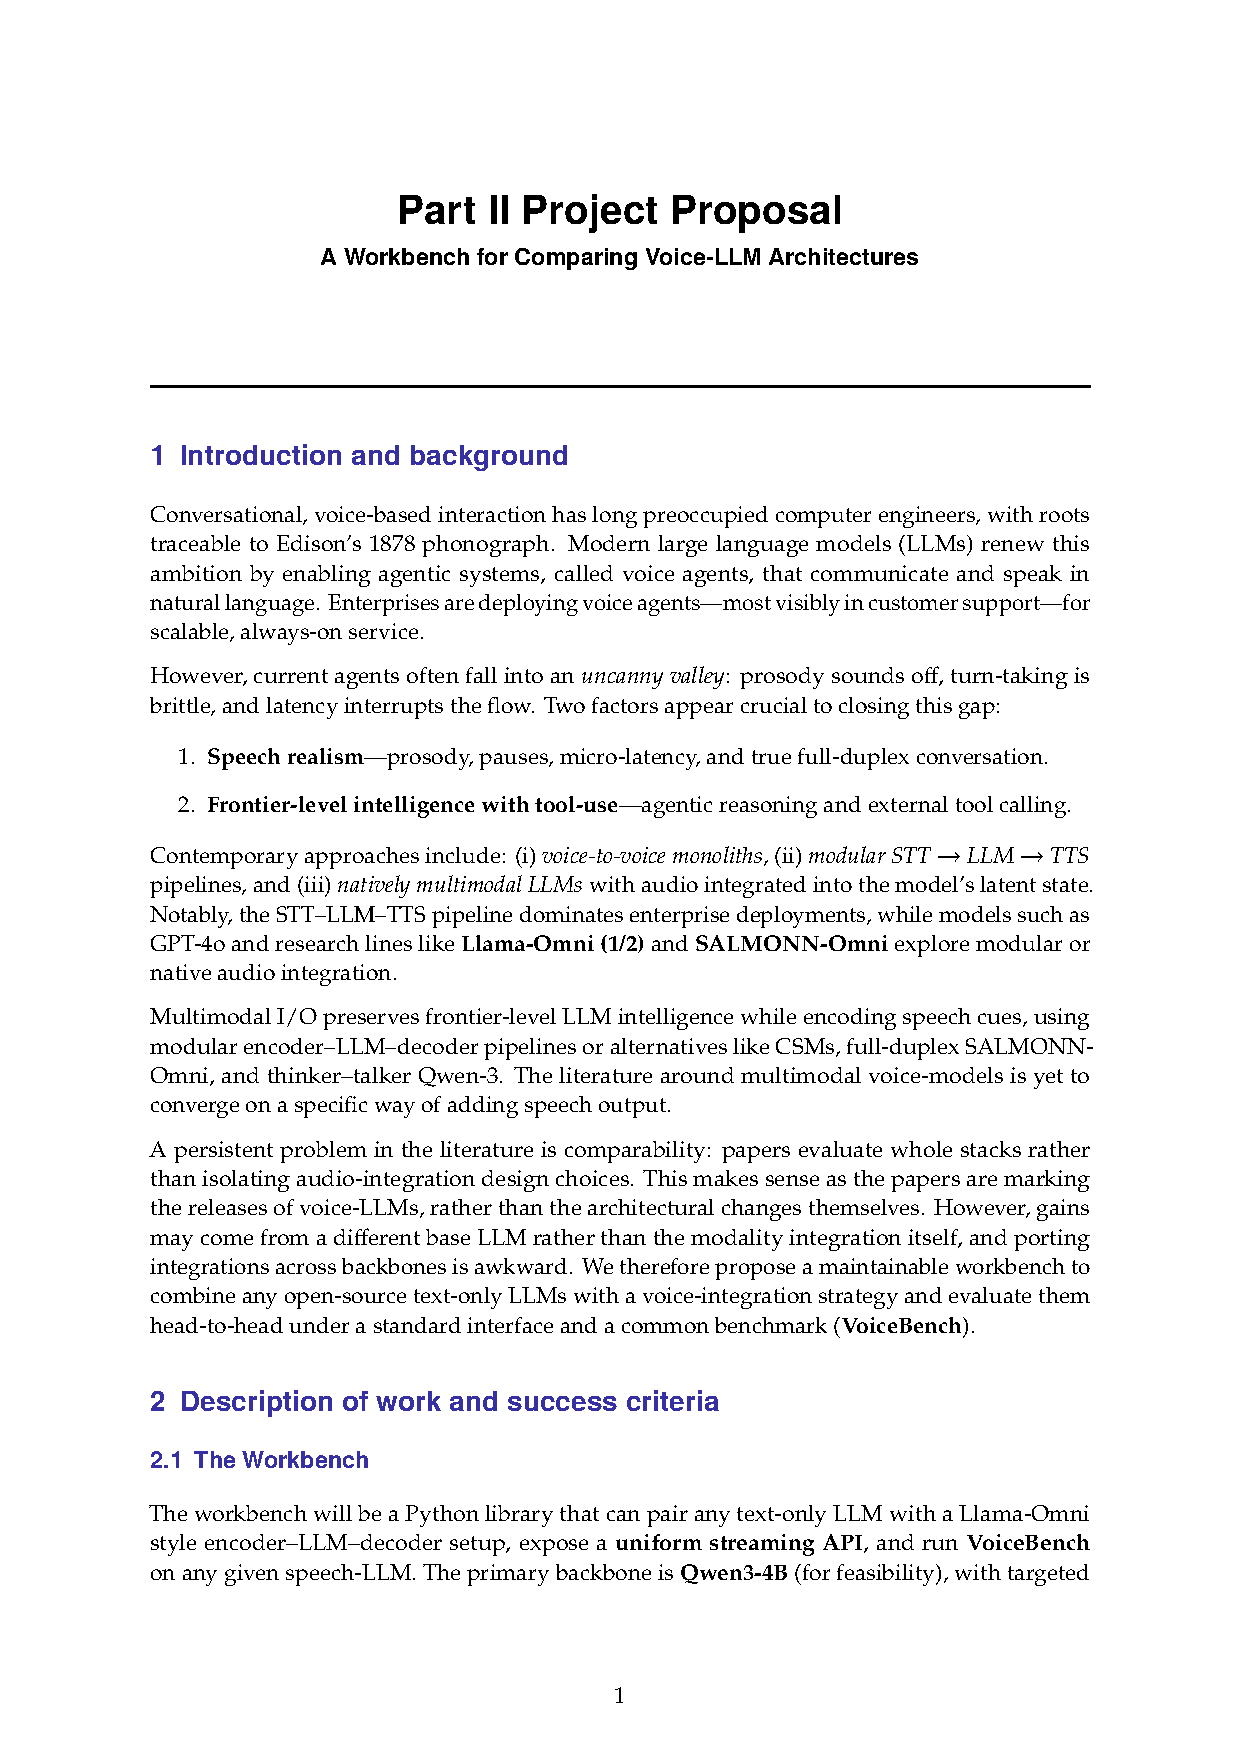
\includegraphics[height=4.8cm,page=1]{project_proposal.pdf}
\end{frame}

\begin{frame}{Current Work: Architecture}
\centering
\vspace{1em}
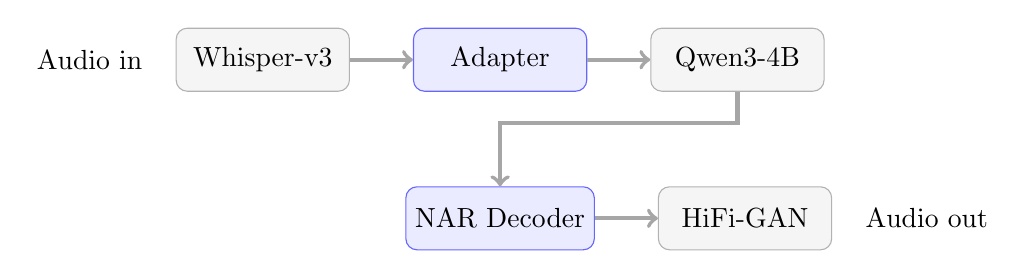
\begin{tikzpicture}[
    node distance=0.6cm and 0.8cm,
    box/.style={rectangle, draw=blue!60, fill=blue!8, rounded corners, 
                minimum width=2.2cm, minimum height=0.8cm, font=\normalsize},
    frozen/.style={rectangle, draw=gray!60, fill=gray!8, rounded corners,
                minimum width=2.2cm, minimum height=0.8cm, font=\normalsize},
    arrow/.style={->, thick, gray!70, line width=1.5pt}
]
    \node[frozen] (whisper) {Whisper-v3};
    \node[box, right=of whisper] (adapter) {Adapter};
    \node[frozen, right=of adapter] (qwen) {Qwen3-4B};
    
    \node[box, below=1.2cm of adapter] (decoder) {NAR Decoder};
    \node[frozen, right=of decoder] (vocoder) {HiFi-GAN};
    
    \draw[arrow] (whisper) -- (adapter);
    \draw[arrow] (adapter) -- (qwen);
    \draw[arrow] (qwen.south) -- ++(0,-0.4) -| (decoder.north);
    \draw[arrow] (decoder) -- (vocoder);
    
    \node[font=\normalsize, left=0.3cm of whisper] {Audio in};
    \node[font=\normalsize, right=0.3cm of vocoder] {Audio out};
\end{tikzpicture}

\vspace{1.5em}
\begin{tabular}{cc}
\textcolor{blue!60}{\rule{1cm}{0.3cm}} Trainable & \textcolor{gray!60}{\rule{1cm}{0.3cm}} Frozen
\end{tabular}

\vspace{1.5em}
\textbf{Two-stage training:} (1) Train adapter with LM loss \quad (2) Train decoder with CTC loss
\end{frame}

\begin{frame}{Encoder Training (Stage 1)}
\centering
\vspace{0.5em}

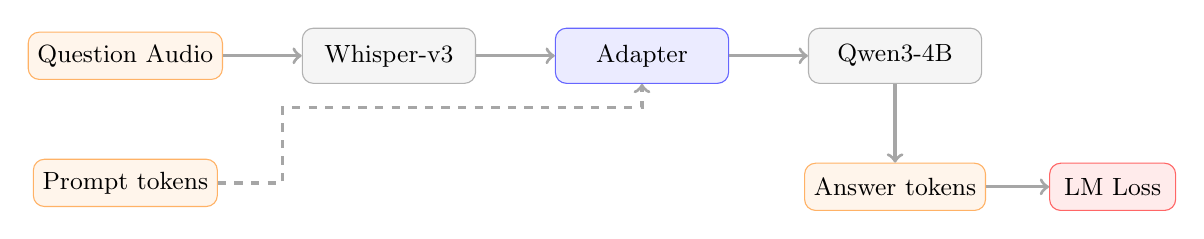
\begin{tikzpicture}[
    node distance=0.5cm and 1cm,
    box/.style={rectangle, draw=blue!60, fill=blue!8, rounded corners, 
                minimum width=2.2cm, minimum height=0.7cm, font=\small},
    frozen/.style={rectangle, draw=gray!60, fill=gray!8, rounded corners,
                minimum width=2.2cm, minimum height=0.7cm, font=\small},
    data/.style={rectangle, draw=orange!60, fill=orange!8, rounded corners,
                minimum width=2cm, minimum height=0.6cm, font=\small},
    arrow/.style={->, thick, gray!70, line width=1.2pt}
]
    \node[data] (audio) {Question Audio};
    \node[frozen, right=of audio] (whisper) {Whisper-v3};
    \node[box, right=of whisper] (adapter) {Adapter};
    \node[frozen, right=of adapter] (qwen) {Qwen3-4B};
    
    \draw[arrow] (audio) -- (whisper);
    \draw[arrow] (whisper) -- (adapter);
    \draw[arrow] (adapter) -- (qwen);
    
    \node[data, below=1cm of audio] (prompt) {Prompt tokens};
    \node[data, below=1cm of qwen] (answer) {Answer tokens};
    
    \draw[arrow, dashed] (prompt) -- ++(2,0) |- ([yshift=-0.3cm]adapter.south) -- (adapter.south);
    \draw[arrow] (qwen) -- (answer);
    
    \node[draw=red!60, fill=red!8, rounded corners, minimum width=1.6cm, minimum height=0.6cm, font=\small, right=0.8cm of answer] (loss) {LM Loss};
    \draw[arrow] (answer) -- (loss);
\end{tikzpicture}

\vspace{1.5em}
\begin{columns}[T]
\begin{column}{0.48\textwidth}
\textbf{What's trained}
\begin{itemize}
\setlength\itemsep{0.3em}
\item[\small$\bullet$] Adapter only (2-layer MLP)
\item[\small$\bullet$] Whisper and Qwen frozen
\item[\small$\bullet$] Maps Whisper dim $\to$ Qwen dim
\end{itemize}
\end{column}
\begin{column}{0.48\textwidth}
\textbf{Loss}
\begin{itemize}
\setlength\itemsep{0.3em}
\item[\small$\bullet$] Standard next-token prediction
\item[\small$\bullet$] Cross-entropy on answer tokens
\item[\small$\bullet$] Teacher forcing
\end{itemize}
\end{column}
\end{columns}
\end{frame}

\begin{frame}{Decoder Training (Stage 2)}
\centering
\vspace{0.3em}

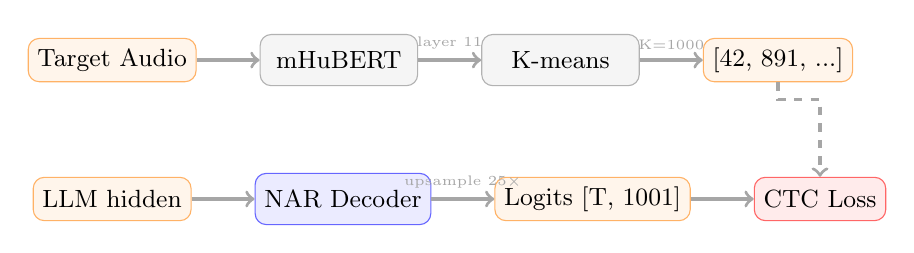
\begin{tikzpicture}[
    node distance=0.5cm and 0.8cm,
    box/.style={rectangle, draw=blue!60, fill=blue!8, rounded corners, 
                minimum width=2cm, minimum height=0.65cm, font=\small},
    frozen/.style={rectangle, draw=gray!60, fill=gray!8, rounded corners,
                minimum width=2cm, minimum height=0.65cm, font=\small},
    data/.style={rectangle, draw=orange!60, fill=orange!8, rounded corners,
                minimum width=1.8cm, minimum height=0.55cm, font=\small},
    arrow/.style={->, thick, gray!70, line width=1.2pt}
]
    \node[data] (targetaudio) {Target Audio};
    \node[frozen, right=of targetaudio] (hubert) {mHuBERT};
    \node[frozen, right=of hubert] (kmeans) {K-means};
    \node[data, right=of kmeans] (units) {[42, 891, ...]};
    
    \draw[arrow] (targetaudio) -- (hubert);
    \draw[arrow] (hubert) -- node[above, font=\tiny] {layer 11} (kmeans);
    \draw[arrow] (kmeans) -- node[above, font=\tiny] {K=1000} (units);
    
    \node[data, below=1.2cm of targetaudio] (hidden) {LLM hidden};
    \node[box, right=of hidden] (decoder) {NAR Decoder};
    \node[data, right=of decoder] (logits) {Logits [T, 1001]};
    \node[draw=red!60, fill=red!8, rounded corners, minimum width=1.6cm, minimum height=0.55cm, font=\small, right=of logits] (ctc) {CTC Loss};
    
    \draw[arrow] (hidden) -- (decoder);
    \draw[arrow] (decoder) -- node[above, font=\tiny] {upsample 25$\times$} (logits);
    \draw[arrow] (logits) -- (ctc);
    \draw[arrow, dashed] (units) -- ++(0,-0.5) -| (ctc.north);
\end{tikzpicture}

\vspace{1em}
\begin{columns}[T]
\begin{column}{0.48\textwidth}
\textbf{Unit extraction} (offline)
\begin{itemize}
\setlength\itemsep{0.25em}
\item[\small$\bullet$] mHuBERT: self-supervised speech repr.
\item[\small$\bullet$] K-means quantizes to 1000 clusters
\item[\small$\bullet$] Deduplicate consecutive repeats
\end{itemize}
\end{column}
\begin{column}{0.48\textwidth}
\textbf{CTC loss}
\begin{itemize}
\setlength\itemsep{0.25em}
\item[\small$\bullet$] No alignment labels available
\item[\small$\bullet$] Sum prob. of \textit{all} valid alignments
\item[\small$\bullet$] Blank token absorbs timing slack
\end{itemize}
\end{column}
\end{columns}

\vspace{0.8em}
{\small\textit{Why sum all alignments?} We don't know which frames map to which units. CTC marginalizes over this uncertainty; any alignment that produces the correct sequence contributes to the loss.}
\end{frame}

\begin{frame}{Current Work: Results}
\begin{columns}[c]
\begin{column}{0.45\textwidth}
\centering
\textbf{Training on H100}

\vspace{1em}
\begin{tabular}{ll}
\toprule
Encoder training & 7.5 hours \\
Decoder training & 16.5 hours \\
\midrule
Encoder val loss & 1.60 \\
Decoder val loss & 0.74 \\
\bottomrule
\end{tabular}

\vspace{1.5em}
Output coherent for 7-8 seconds, then degrades.

\vspace{0.5em}
Decoder undersized: 1024 vs 4096 hidden dim.
\end{column}

\begin{column}{0.5\textwidth}
\centering
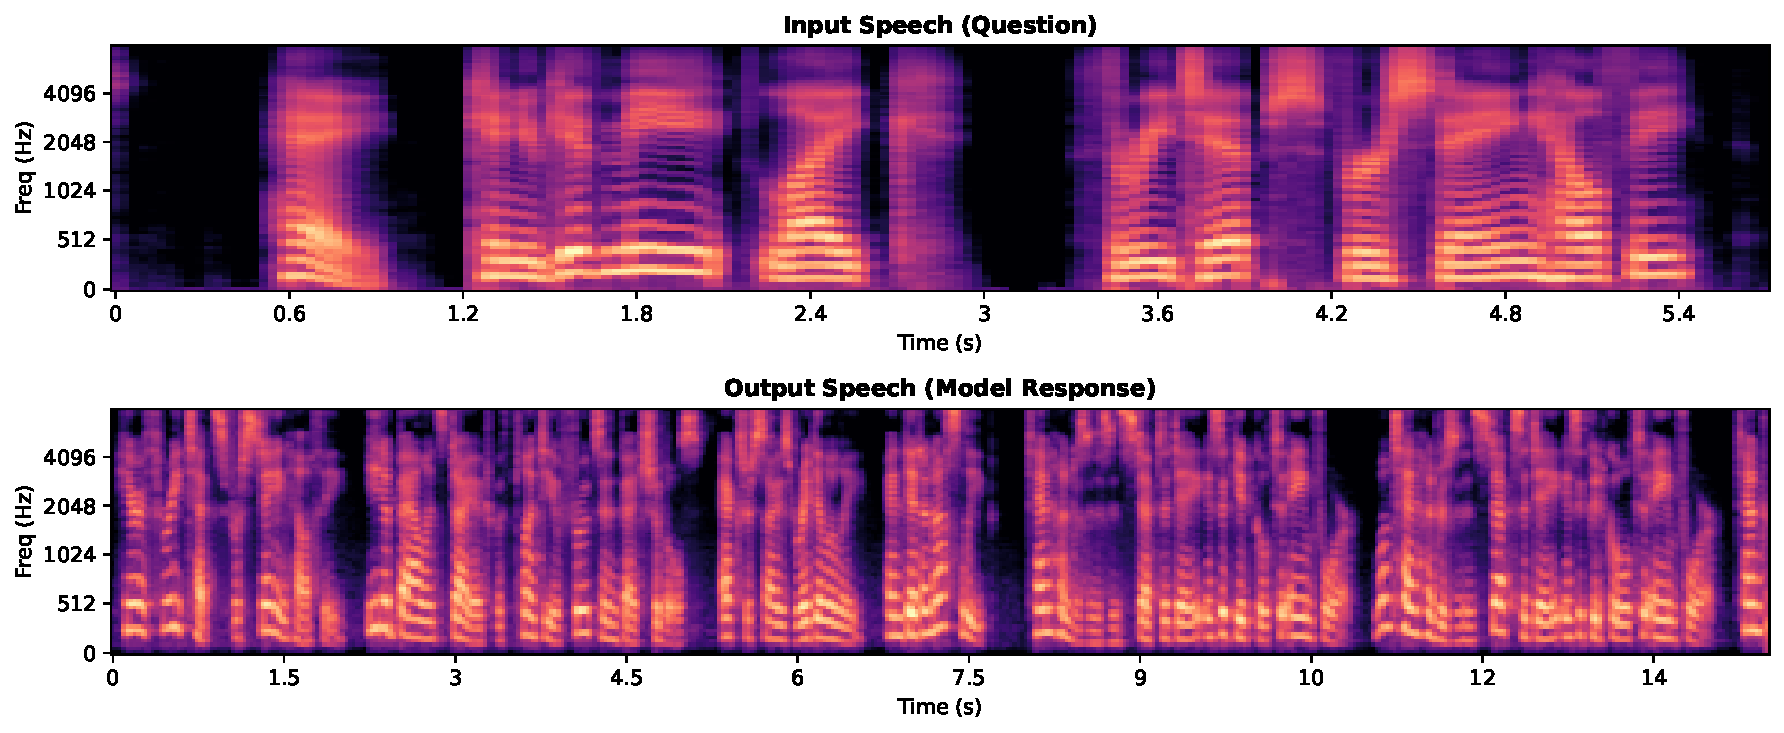
\includegraphics[width=\textwidth]{input_output_comparison.pdf}

\vspace{0.3em}
{\small Input (top) vs output (bottom) spectrograms}
\end{column}
\end{columns}
\end{frame}

\begin{frame}{Architectural Design}
\centering
Splitting the codebase into \textbf{product} and \textbf{research}.

\vspace{1.5em}
\begin{columns}[T]
\begin{column}{0.45\textwidth}
\centering
\textbf{Product}

\vspace{0.5em}
\begin{tabular}{l}
\toprule
Pick voice, dataset, base model \\
Kick off training via API \\
Serve models (serverless) \\
Run VoiceBench evaluations \\
\midrule
FastAPI, Modal, S3, open-source TTS \\
\bottomrule
\end{tabular}
\end{column}

\begin{column}{0.45\textwidth}
\centering
\textbf{Research}

\vspace{0.5em}
\begin{tabular}{l}
\toprule
Run ablations \\
Try new architectures \\
Measure quality \\
\\
\midrule
SkyPilot, Hydra, WandB \\
\bottomrule
\end{tabular}
\end{column}
\end{columns}
\end{frame}

\begin{frame}{Timeline}
\vspace{0.5em}
\centering
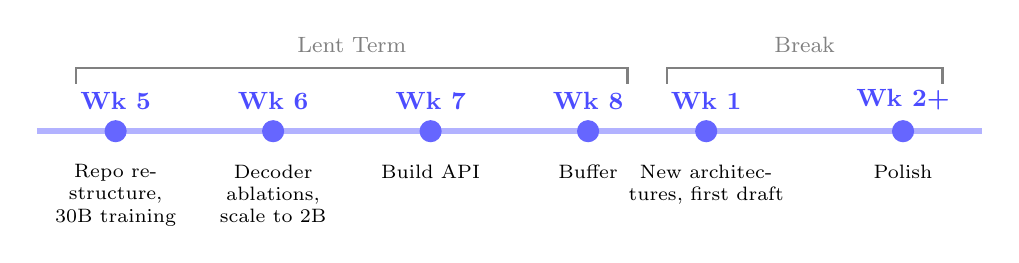
\begin{tikzpicture}
    % Main timeline
    \draw[line width=2pt, blue!30] (0,0) -- (12,0);
    
    % Lent term bracket
    \draw[thick, gray] (0.5, 0.6) -- (0.5, 0.8) -- (7.5, 0.8) -- (7.5, 0.6);
    \node[font=\footnotesize, gray] at (4, 1.1) {Lent Term};
    
    % Break bracket  
    \draw[thick, gray] (8, 0.6) -- (8, 0.8) -- (11.5, 0.8) -- (11.5, 0.6);
    \node[font=\footnotesize, gray] at (9.75, 1.1) {Break};
    
    % Week markers and content
    \foreach \x/\week/\tasks in {
        1/5/{Repo restructure, 30B training},
        3/6/{Decoder ablations, scale to 2B},
        5/7/{Build API},
        7/8/{Buffer},
        8.5/1/{New architectures, first draft},
        11/2+/{Polish}
    } {
        \fill[blue!60] (\x, 0) circle (4pt);
        \node[font=\small\bfseries, blue!70, above] at (\x, 0.15) {Wk \week};
        \node[font=\scriptsize, text width=2cm, align=center, below] at (\x, -0.3) {\tasks};
    }
\end{tikzpicture}

\vspace{1.5em}
\textbf{12 weeks to deadline}
\end{frame}

\begin{frame}{Reflections}
\begin{itemize}
    \setlength\itemsep{0.8em}
    \item SkyPilot + Hydra + WandB makes ablations a single command
    \item Writing gets to 80\% fast; the last 20\% takes just as long
    \item Original plan targeted ICLR workshop deadlines; submitted different work there instead
    \item GPU quotas were painful early on, now have A100 clusters, H100s coming
    \item Still somewhat capital-constrained
    \item Key decision: how deep to go on infrastructure? Modal gives autoscaling but costs money. Custom is cheaper but more work.
\end{itemize}
\end{frame}

\end{document}
